\section{Cel przeglądu}\label{chapter:cel_przegladu}

Celem przeglądu jest poznanie obecnego stanu wiedzy oraz wykorzystanie jej jako wsparcia w odpowiedzi na postawione w pracy pytania badawcza. 
Zamierzeniem przeglądu jest analiza trzech głównych obszarów:

\begin{enumerate}
    \item Czynników wpływających na wydajność AWS Lambda.
    \item Istniejących metod optymalizacji wydajności AWS Lambda dla ekosystemu Java.
    \item Charakterystyki rozwoju funkcji AWS Lambda z perspektywy pracy programisty.
\end{enumerate}

Obszary te zostały wybrane na podstawie pytań badawczych. 
Ich zrozumienie pozwoli na identyfikację zagadnień, które nie zostały wystarczająco zbadane, 
a mogą zawierać potencjalne metody usprawnienia wydajności funkcji AWS Lambda w ramach ekosystemu Java.
Dodatkowo, pozwoli to na przygotowanie badań, które będą lepiej odzwierciedlać rzeczywistą praktykę aplikacji bezserwerowych.

\section{Metodyka przeglądu literatury}\label{chapter:metodyka_przegladu}

Do wykonania przeglądu literatury wybrano metodykę szybkiego przeglądu (ang. rapid review). 
Szybkie przeglądy to metoda badań wtórnych stosowana w inżynierii oprogramowania, której celem jest szybka synteza wyników badań.
Ich głównym zadaniem jest dostarczanie aktualnych informacji opartych na dowodach.
Pomaga to praktykom podejmować decyzje dotyczące specyficznych problemów w ramach ich kontekstu pracy i ograniczeń czasowych.
Metoda ta często wykonywana jest przez jedną osobę, przy jednoczesnym użyciu bardziej restrykcyjnych kryteriów.
Jest to jednak świadoma strategia mająca na celu redukcję czasu i wysiłku \cite{cartaxo2020rapidreviewssoftwareengineering}.
Proces szybkiego przeglądu składa się z trzech etapów, które zostały zrealizowane w pracy:

\begin{enumerate}
    \item Zaplanowanie (określenie potrzeby przeglądu, problemu i pytań badawczych).
    \item Przeprowadzenie (stworzenie i wykonanie strategi wyszukiwania, procedur selekcji, oceny jakości, ekstrakcji i syntezy).
    \item Raportowanie (omówienie wyników przeglądu i odpowiedź na pytania badawcze).
\end{enumerate}

\section{Proces przeglądu}\label{chapter:proces_przegladu}

\subsection{Omówienie pytań badawczych}\label{chapter:omowanie_pytan_badawczych}

Formułowanie pytań badawczych to istotna część przeglądu \cite{KitchenhamProceduresSR}. 
Pytania te, oparte na celu pracy, wskazują kierunek przy opracowywaniu i wdrażaniu kryteriów przeglądu. 
W ramach wykonanego przeglądu literatury postawiono konkretne pytania, mające na celu ukierunkowanie analizy, 
co umożliwi odpowiedź na główne pytania badawcze całej pracy. 
Do każdego z nich dołączono krótkie wyjaśnienie i motywację.
 
\begin{itemize}
    \item PB1: Jakie są główne czynniki wpływające na wydajność funkcji AWS Lambda?
    
    Odpowiedź na postawione pytanie ma na celu zrozumienie sposobu działania AWS Lambda pod kątem wydajności.
    Powyższe pytanie nie odnosi się wyłącznie do technologii z środowiska Java, co pozwoli na poszerzenie analizy.
    Dostarczone odpowiedzi będą wsparciem dla znalezienia nowych metod optymalizacji wydajności, ze względu na zrozumienie na jakie czynniki owe metody mogą wpływać.
    Dodatkowo, zidentyfikowane czynniki pozwolą na przygotowanie bardziej jakościowych badań. 
    Badania będą mogły być realizowane w ramach różnych scenariuszy, które będą wykonane dla różnych wartości znalezionych parametrów.  

    \item PB2: Jakie są istniejące metody optymalizacji wydajności funkcji AWS Lambda działających w ekosystemie Java?
    
    Pytanie pozwoli ustalić jaki jest istniejący stan wiedzy dla metod optymalizacji wydajności funkcji AWS Lambda w ramach środowiska Java.
    W ramach tego pytania analiza skupi się na szeroko pojętym ekosystemie Java, czyli różnych językach wywodzących się z Javy, bibliotekach, frameworkach i środowiskach wykonawczych.
    Analiza pozwoli na wskazanie obszarów, które nie zostały jeszcze zbadane lub zostały zbadane niewystarczająco.
    Tak wyznaczone zagadnienia będą potencjalnym miejscem poszukiwania nowych metod.
    Stanowi to znaczącą pomoc w realizacji celu pracy.

    \item PB3: Jakie są cechy rozwoju aplikacji w architekturze bezserwerowej AWS Lambda?
    
    Ostatnie pytanie skupia się na perspektywie programisty tworzącego aplikacje opierające się o funkcje bezserwerowe oferowane przez AWS.
    Zdecydowano się na przegląd literatury w tym zakresie ze względu na specyficzne podejście do tworzenia takich aplikacji.
    Rozpatrzenie tego pozwoli następnie na analizę zaproponowanych metod optymalizacji pod względem ich wpływu na proces wytwarzania oprogramowania.
    Przewiduje się, że analiza ta może być skomplikowana z powodu zróżnicowanych praktyk budowy wspomnianych systemów.

\end{itemize}

\subsection{Przeszukiwane zasoby}\label{chapter:przeszukiwane_zasoby}

\subsubsection{Biblioteki cyfrowe}

Głównymi źródłami informacji, które zostały przeszukane były biblioteki cyfrowe IEEE oraz Scopus. 
Wybór bibliotek był podyktowany dostępnością w e-zasobach Politechniki Wrocławskiej. 
Kluczową cechą wybranych bibliotek była możliwość użycia operatorów logicznych i wyszukiwania słów kluczowych w konkretnych elementach pracy.
W ramach pierwszych iteracji stwierdzono potrzebę ich użycia ze względu na obszerność tematów bezserwerowych, co opisano w dalszej części pracy.

\subsubsection{Szara literatura}

W celu uwzględnienia w przeglądzie szarej literatury zdecydowano się na użycie wyszukiwarki Google Scholar.
W procesie użyto zapytań odpowiednio dostosowanych do wyszukiwarki, gdzie przeszukiwano tytuł, abstrakt oraz pełny tekst pracy.

Rekomendacje w zakresie włączania szarej literatury do systematycznych przeglądów wyznaczyli Kitchenham, Madeyski i Budgen \cite{9754223}.
Podkreślają oni jendak, aby wyraźnie rozróżnić informacje uzyskane z źródeł zgodnych z definicją ,,Prague'' a innych zasobów internetowych (jak np. blogi).
W ramach przeglądu przeszukiwano dodatkowe materiały internetowe, które posłużyły jako wsparcie wyjaśnienia poszczególnych metod optymalizacji.
Nie zostały one jednak włączone bezpośrednio do wyników przeglądu.

\subsection{Wyszukiwane terminy}\label{chapter:wyszukiwane_terminy}

Istotnym elementem strategii wyszukiwania było stworzenie odpowiednich zapytań dla wyszukiwarek. 
Zostały one przygotowane na bazie postawionych pytań badawczych do przeglądu literatury.
Każde zapytanie zostało przygotowane według poniższego procesu:

\begin{enumerate}
    \item Wyznaczenie słów kluczowych na bazie pytania badawczego, gdzie słowa kluczowe definiują odpowiednie domeny \cite{doi:10.1177/0739456X17723971}.
    Pozwoliło to na wykonanie pierwszych prób wyszukiwania, co pozwoliło na późniejsze dostosowanie zapytań i użycie odpowiednich filtrów oferowanych przez wyszukiwarki.
    Wszystkie słowa kluczowe zostały przedstawione w języku polskim i angielskim.
    \item Dla każdego słowa kluczowego określono synonimy i wyrazy bliskoznaczne. Tam gdzie to możliwe terminy zostały zawarte zarówno w liczbie mnogiej jak i pojedynczej.
    \item Połączono terminy odpowiednimi operatorami logicznymi. Synonimy i wyrazy bliskoznaczne zostały połączone operatorami OR, a poszczególne ich grupy AND.
    \item Dostosowano wyszukiwania fraz aby obejmowały elementy pracy, jak: słowa kluczowe, tytuł, abstrakt oraz pełny tekst (w miarę dostępności dla wyszukiwarki).
\end{enumerate}

\subsubsection*{Ustalenie słów kluczowych}

Dla każdego pytania badawczego ustalono zbiór pytań kluczowych:

\begin{itemize}
    \item PB1: ,,Jakie są główne czynniki wpływające na wydajność funkcji AWS Lambda?''
    \begin{itemize}
        \item W języku polskim: czynniki, wydajność, AWS Lambda
        \item W języku angielskim: factors, performance, AWS Lambda
    \end{itemize}
    \item PB2: ,,Jakie są istniejące metody optymalizacji wydajności funkcji AWS Lambda działających w ekosystemie Java?''
    \begin{itemize}
        \item W języku polskim: optymalizacja, wydajność, AWS Lambda, Java
        \item W języku angielskim: optimization, performance, AWS Lambda, Java
    \end{itemize}
    \item PB3: ,,Jakie są cechy rozwoju aplikacji w architekturze bezserwerowej AWS Lambda?''
    \begin{itemize}
        \item W języku polskim: rozwój oprogramowania, AWS Lambda, model bezserwerowy
        \item W języku angielskim: software development, AWS Lambda, serverless
    \end{itemize}
\end{itemize}

\subsubsection*{Ustalenie synonimów i wyrazów bliskoznacznych}

Dla każdego słowa kluczowego ustalono synonimy, wyrazy bliskoznaczne i powiązane terminy. 
Zostały one określone poprzez iteracyjne testowanie kolejnych terminów.
Słowo kluczowe ,,AWS Lambda'' zostało rozdzielone na dwa pojęcia: AWS oraz Lambda.
Wynika to z różnych użyć tych terminów w wyszukiwanych pracach.

Opracowane słowa kluczowe z powiązanymi terminami:

\begin{itemize}
    \item PB1:
    \begin{itemize}
        \item \textbf{factors}: factor, factors, aspect, aspects, component, components, parameter, parameters, influence, influences, consideration, considerations
        \item \textbf{performance}: performance, efficiency, effectiveness, speed, throughput, responsiveness, latency, execution time, processing time, productivity, computational efficiency, optimization
        \item \textbf{AWS}: AWS, Amazon
        \item \textbf{Lambda}: Lambda, FaaS, Function-as-a-Service, serverless function, serverless functions, cloud function, cloud functions
    \end{itemize}
    \item PB2:
    \begin{itemize}
        \item \textbf{optimization}: optimization, optimisation, optimizing, improve, improvement, improving, method, methods, strategy, strategies, approach, approaches, technique, techniques, procedure, procedures, practice, practices, mechanism, mechanisms, solution, solutions, pattern, patterns
        \item \textbf{performance}: performance, efficiency, effectiveness, speed, throughput, responsiveness, latency, execution time, processing time, delay, warm start, cold start
        \item \textbf{Java}: Java, JVM, Java Virtual Machine, JDK, Kotlin, Scala, GraalVM, Spring, SpringBoot
        \item \textbf{AWS}: AWS, Amazon
        \item \textbf{Lambda}: Lambda, FaaS, Function as a Service, serverless function, serverless functions
    \end{itemize}
    \item PB3:
    \begin{itemize}
        \item \textbf{software development}: development process, development workflow, development lifecycle, software development, developing, software engineering, developer experience, patterns
        \item \textbf{serverless}: serverless
        \item \textbf{Lambda}: Lambda, FaaS, Function as a Service, serverless function, serverless functions
        \item \textbf{AWS}: AWS, Amazon
    \end{itemize}
\end{itemize}

\subsubsection*{Opracowane zapytania}

Na bazie słów kluczowych i pozwiązanych z nimi terminów opracowano poniższe zapytania:

\begin{itemize}
    \item PB1:

    (,,factor'' OR ,,factors'' OR ,,aspect'' OR ,,aspects'' OR ,,component'' OR ,,components'' OR ,,parameter'' OR ,,parameters'' OR ,,influence'' OR ,,influences'' OR ,,consideration'' OR ,,considerations'') 
    AND (,,performance'' OR ,,efficiency'' OR ,,effectiveness'' OR ,,speed'' OR ,,throughput'' OR ,,responsiveness'' OR ,,latency'' OR ,,execution time'' OR ,,processing time'' OR ,,productivity'' OR ,,computational efficiency'' OR ,,optimization'') 
    AND (,,Lambda'' OR ,,FaaS'' OR ,,Function as a Service'' OR ,,serverless function'' OR ,,serverless functions'' OR ,,cloud function'' OR ,,cloud functions'')
    AND (,,AWS'' OR ,,Amazon'')

    \item PB2:
    
    (,,optimization'' OR ,,optimisation'' OR ,,optimizing'' OR ,,improve'' OR ,,improvement'' OR ,,improving'' OR ,,method'' OR ,,methods'' OR ,,strategy'' OR ,,strategies'' OR ,,approach'' OR ,,approaches'' OR ,,technique'' OR ,,techniques'' OR ,,procedure'' OR ,,procedures'' OR ,,practice'' OR ,,practices'' OR ,,mechanism'' OR ,,mechanisms'' OR ,,solution'' OR ,,solutions'' OR ,,pattern'' OR ,,patterns'')
    AND (,,performance'' OR ,,efficiency'' OR ,,effectiveness'' OR ,,speed'' OR ,,throughput'' OR ,,responsiveness'' OR ,,latency'' OR ,,execution time'' OR ,,processing time'' OR ,,delay'' OR ,,warm start'' OR ,,cold start'')
    AND (,,Java'' OR ,,JVM'' OR ,,Java Virtual Machine'' OR ,,JDK'' OR ,,Kotlin'' OR ,,Scala'' OR ,,GraalVM'' OR ,,Spring'' OR ,,SpringBoot'')
    AND (,,Lambda'' OR ,,FaaS'' OR ,,Function as a Service'' OR ,,serverless function'' OR ,,serverless functions'')
    AND (,,AWS'' OR ,,Amazon'')

    \item PB3:
    
    (,,serverless'') 
    AND (,,development process'' OR ,,development workflow'' OR ,,development lifecycle'' OR ,,software development'' OR ,,developing'' OR ,,software engineering'' OR ,,developer experience'' OR ,,patterns'') 
    AND (,,Lambda'' OR ,,FaaS'' OR ,,Function as a Service'' OR ,,serverless function'' OR ,,serverless functions'') 
    AND (,,AWS'' OR ,,Amazon'')
    
\end{itemize}

W pierwszych wyszukaniach z użyciem powyższych zapytań zauważono, że znacząca część wyników nie odnosi się do serwisu AWS Lambda, na którym skupia się praca.
Wyniki te odnosiły się przeważnie do innych usług lub platform bezserwerowych (np. OpenWhisk).
Z tego powdou zdecydowano się na zawężenie wyników poprzez dodanie wymogu występowania terminów AWS i Lambda (oraz ich powiązanych terminów) w tytule lub abstrakcie.
W wyszukaniach IEEE oraz Scopus warunek ten został dodany do istniejącej części zapytania. 
W wyszukiwarce Google Scholar, została dodana część wyszukująca jakikolwiek z powiązanych terminów z obu tych grup w tytule. 

\subsection{Selekcja literatury}\label{chapter:selekcja_literatury}

W celu ograniczenia liczby analizowanych prac i zgromadzić badania niezbędne do dalszych analiz, określono poniższe kryteria włączenia oraz wyłączenia pozycji literaturowych \cite{cartaxo2020rapidreviewssoftwareengineering}:
\begin{itemize}
    \item praca została opublikowana w 2014 roku lub później - jest to rok kiedy po raz pierwszy zaprezentowano AWS Lambda, zatem założono, że prace jej temat nie zostały napisane wcześniej,
    \item praca zawiera się w dziedzinie informatyki (ang. computer science) lub inżynierii oprogramowania (ang. software engineering)
    \item praca została napisana w języku angielskim
    \item duplikaty pomiędzy poszczególnymi wyszukiwarkami oraz frazami nie są włączane do przeglądu literatury 
\end{itemize}

\begin{figure}[h]
    \centering
    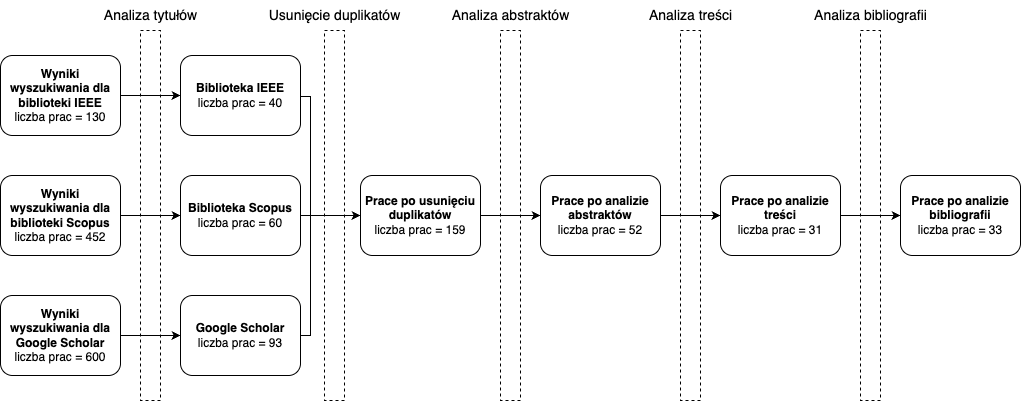
\includegraphics[width=0.95\textwidth]{charts/literature_review_process.drawio.png}
    \caption{Proces selekcji literatury [źródło: opracowanie własne]}
    \label{fig:literature_review_process}
\end{figure}

\begin{table}[h!]
    \caption{Liczba wybranych prac w zależności od etapu selekcji [źródło: opracowanie własne]}
    \centering
    \renewcommand{\arraystretch}{1.3}
    \begin{tabular}{|>{\centering\arraybackslash}m{1cm}|>{\centering\arraybackslash}m{1.7cm}|>{\centering\arraybackslash}m{1.7cm}|>{\centering\arraybackslash}m{1.6cm}|>{\centering\arraybackslash}m{1.7cm}|>{\centering\arraybackslash}m{1.7cm}|>{\centering\arraybackslash}m{1.6cm}|>{\centering\arraybackslash}m{1.7cm}|}
    \hline
    \scriptsize\textbf{} & \scriptsize\textbf{} & \multicolumn{6}{c|}{\scriptsize\textbf{Liczba prac po zakończeniu danego etapu}} \\
    \cline{3-8}
    \scriptsize\textbf{Fraza} & \scriptsize\textbf{Biblioteka cyfrowa} & \scriptsize\textbf{Wyszukanie} & \scriptsize\textbf{Analiza tytułów} & \scriptsize\textbf{Usunięcie duplikatów} & \scriptsize\textbf{Analiza abstraktów} & \scriptsize\textbf{Analiza treści} & \scriptsize\textbf{Snowballing} \\
    \hline
    \multirow{3}{*}{1} & IEEE           & 59    & 17 & 17 & 12 & 8 & 8 \\
    \cline{2-8}
                       & Scopus         & 217 (200)    & 17  & 15  & 5  & 3  & 4  \\
    \cline{2-8}
                       & Google Scholar & 4050 (200)  & 50 & 40 & 9 & 4 & 4 \\
    \hline
    \multirow{3}{*}{2} & IEEE           & 8           & 4  & 4  & 4  & 4  & 5  \\
    \cline{2-8}
                       & Scopus         & 52    & 9  & 6  & 3  & 3  & 3  \\
    \cline{2-8}
                       & Google Scholar & 1550 (200)   & 26 & 23  & 6  & 2  & 2  \\
    \hline
    \multirow{3}{*}{3} & IEEE           & 63           & 19  & 15  & 5  & 3  & 3  \\
    \cline{2-8}
                       & Scopus         & 205 (200)    & 34  & 23  & 3  & 2  & 2  \\
    \cline{2-8}
                       & Google Scholar & 397 (200)  & 17  & 16  & 5  & 2  & 2  \\
    \hline
    \multicolumn{2}{|c|}{\textbf{Suma}} & \textbf{1182} & \textbf{193} & \textbf{159} & \textbf{52} & \textbf{31} & \textbf{33} \\
    \hline
    \end{tabular}
    \label{table:review_process_table}
\end{table}


Wcześniej opracowane zapytania zostały użyte do wyszukań w poszczególnych wyszukiwarkach. 
Dla prac wyszukanych w poszczególnych wyszukiwarkach, został zastosowany proces selekcji.
Liczba prac w poszczególnych etapach procesu została przedstawiona w Tabeli \ref{table:review_process_table}.
Dodatkowo, zobrazowano proces selekcji na Rysunku \ref{fig:literature_review_process}.

W przypadku, gdy dla danej frazy wyszukiwania odnaleziono więcej niż 200 publikacji, do dalszej analizy kwalifikowano pierwszych 200 pozycji, posortowanych według malejącej trafności.
Następnie, każda z tych prac była poddawana procesowi selekcji, który polegał na poddaniu kryteriom włączenia i wyłączenia, analizie tytułów, abstraktów i treści.
Jeśli praca została włączona do przeglądu literatury, dokonywano analizy jej bibliografii, wykorzystując metodę kuli śnieżnej (ang. snowballing sampling method) \cite{10.1214/aoms/1177705148}.
Artykuły włączone w ten sposób do przeglądu zostały przypisane do frazy, z której pochodziła pierwotna praca.

Dla każdej pracy naukowej, która została włączona do przeglądu literatury, przygotowano odpowiedni wpis w formacie BibTeX, umożliwiający jej późniejsze zacytowanie. 
Zapytania do bibliotek cyfrowych zostały wykonane w dniu 8 kwietnia 2025 roku. 

\subsection{Ocena jakości}\label{chapter:ocena_jakosci}

Ważnym elementem przeglądu literatury jest ocena jakości badanych prac.
W przypadku metody szybkiego przeglądu etap ten może zostać pominięty.
Jednak jak zaznacza Cartaxo i inni autorzy \cite{cartaxo2020rapidreviewssoftwareengineering}, etap ten może zostać pomięty, jednak zagrożenia z tym związane powinny zostać jasno wskazane.
W ramach przeglądu zdecydowano się na wykonanie podstawowej oceny jakości.
Dokonanie oceny pozwoli rozpoznać prace, które realizują postawiony w nich cel oraz odpowiadają na sformułowane pytania badawcze.
Dodatkowo, jak podkreślają Madeyski i Kitchenham \cite{wouldWiderAdoption}, istotna jest także możliwość reprodukcji badań.
Niemożliwe do odtworzenia badania mogą prowadzić do znacznych problemów, zatem wynikiem badań powinna być praca oraz powiązane z nią środowisko badawcze.
W ramach procesu oceny zdecydowano się ocenić prace pod kątem trzech kryteriów:

\begin{itemize}
    \item QA1: Czy w pracy postawiono jasny cel?
    \item QA2: Czy w pracy zawarto wyniki, które były wystarczające na poparcie wniosków?
    \item QA3: Czy praca dostarcza wystarczających instrukcji do odtworzenia badań?
\end{itemize}

Każda praca została zbadana pod kątem powyższych pytań.
Na pierwsze i drugie pytanie odpowiedziano tak lub nie, co skutkowało przypisaniem 1 lub 0 punktów.
Dla trzeciego pytania przyjęto trzystopniową skalę oceniającą możliwość reprodukcji badań: nieodtwarzalne (0 punktów), częściowo odtwarzalne (1 punkt), w pełni odtwarzalne (2 punkty).
Badanie uznawano za nieodtwarzalne, gdy praca opisywała jedynie ogólną koncepcję, bez podania kluczowych informacji (np. użytych narzędzi).
Praca była częściowo odtwarzalna, jeśli dostarczała wielu szczegółów ale wciąż wymagała od badacza przyjęcia własnych założeń (np. pomijając wersje bibliotek lub rozmiar pamięci funkcji Lambda).
Najwyższą ocenę przyznawano pracom w pełni odtwarzalnym, które zawierały wszystkie elementy do dokładnego powtórzenia badania, najczęściej poprzez udostępnienie kodu źródłowego w publicznym repozytorium.
Ostatecznie praca była oceniana jako procent zdobytych punktów względem wszystkich możliwych do zdobycia (czyli cztery).
Ocena jakości poszczególnych prac zostały przedstawione w Tabeli \ref{table:research_papers_results}.
